\documentclass[twoside, letterpaper]{report}
\usepackage{geometry}
\usepackage{titlesec}
\usepackage{listings}
\usepackage{xcolor}
\usepackage{titling}
\usepackage{indentfirst}
\usepackage{graphicx}
\usepackage{amsmath}
\usepackage{gensymb}

\newcommand{\subtitle}[1]{%
  \posttitle{%
    \par\end{center}
    \begin{center}\large#1\end{center}
    \vskip0.5em}%
}

\setlength\aftertitleunit{\baselineskip}
\titleformat{\chapter}[display]
  {\normalfont\Huge \scshape}{}{-33pt}{\Huge}
\titleformat{name=\chapter,numberless}[display]
  {\normalfont\Huge \scshape}{}{-33pt}{\Huge}
\titlespacing*{\chapter}{0pt}{50pt}{*2}

\lstdefinestyle{customvhd}{
  belowcaptionskip=1\baselineskip,
  breaklines=true,
  xleftmargin=\parindent,
  language=VHDL,
  showstringspaces=false,
  basicstyle=\footnotesize\ttfamily,
  keywordstyle=\bfseries\color{green!40!black},
  commentstyle=\itshape\color{purple!40!black},
  identifierstyle=\color{blue},
  stringstyle=\color{orange},
}

\makeatletter
 \def\@textbottom{\vskip \z@ \@plus 1pt}
 \let\@texttop\relax
\makeatother

\author{Michael Nickelson}
\title{Final Project}
\subtitle{16.575 - FPGA Logic Design Techniques}
\date{December 4, 2014}

\begin{document}
\maketitle
\newpage\null\thispagestyle{empty}\newpage
\pagenumbering{roman}
\setcounter{page}{1}
\tableofcontents
\cleardoublepage

\chapter{Summary}
\pagenumbering{arabic}
\setcounter{page}{1}

This project implements Conway's Game of Life in VHDL. It is targeted for use on the Altera Cyclone IV as present in the DE-0 Nano development board.

The implementation includes a top-level Game of Life module which implements a block of VRAM, a VGA Controller, and an update element. Within the VRAM there is a block RAM pulled from the Altera superfunction library. Inside the VGA Controller are two parameterized counters to produce hSync and vSync, and a clock divider to provide a 25MHz enable signal to the counters. The block diagram of this setup can be seen in Figure~\ref{fig:block}.
\newline
\par
The VGA controller used is the same as what was developed for HW5 with the only change being delay of hSyncL\_O, vSyncL\_O, vidEnable\_O, and newFrame\_O to work with the RAM block.
\newline
\par
The memory block itself is imported from Altera's mega function library so the source is not included. The parameters used for generation are a 32bit by 2048 line, unregistered, two port RAM.

The memory is initialized using an mif file. In this instance the stored data is a single blinker. I have chosen this shape as it is easy to verify using waveforms and it demonstrates all of the possible cellular activities (survival, death, and birth).
\newline
\par
The update logic is implemented as a state machine (Figure~\ref{fig:state}) which waits in an idle state until the current configuration has been displayed a set number of times. This value is set up as a generic which is passed at instantiation and can allow up to 1s between updates.
There is room for improvement in the implementation of the state machine, particularly the transition from updating back to the idle state. However, given the time constraints of this project the focus was on functionality.

To calculate the next step, golUpdate.vhd uses four 256-bit registers. One each to represent the current states of the last, current, and next lines to be calculated and the next state of the current line. Once these registers are loaded the next state of each bit in the current line is calculated based on the state of its 8 neighbors. This value is saved back to the updatedLine register. This register is then loaded back into RAM in the addresses of the original line. Once the last line is updated the system returns to the idle state.
\newline
\par
The testbench generates a clock and sends reset to the system then allows the system to run with no further input.
\newline
\par
There is a small amount of I/O so pin selection is not terribly complicated. The clock input is determined by the FPGA itself and is located at pin R8. For reset one of the available pushbuttons is used. It is located at pin J15. The outputs hSync, vSync, and pixel are chosen from pins available at the GPIO header. Pins A3, C3, and D3 have been chosen. These 3 are all available on bank 8.

The intent was to select pins compatible with the Papilio VGA Wing available from Sparkfun Electronics (https://www.sparkfun.com/products/11569) unfortunately due to a mechanical incompatibility and the fact that I do not have a monitor to experiment with, this project has been tested in simulation only.
\newline
\par
Figures~\ref{fig:blinker1} through~\ref{fig:blinker4} show a complete cycle of the blinker that is initialized in memory. It alternates between a 3x1 line segment and a 1x3 line segment and is situated in the top left corner of the screen for convenience.
\newline
\par
The total chip utilization is shown below:
\newline
\par
Family	Cyclone IV E

Device	EP4CE22F17C6

Total logic elements	1,762 / 22,320 ( 8 \% )

Total combinational functions	1,537 / 22,320 ( 7 \% )

Dedicated logic registers	1,123 / 22,320 ( 5 \% )

Total registers	1123

Total pins	5 / 154 ( 3 \% )

Total memory bits	65,536 / 608,256 ( 11 \% )
\newline
\par
At 85\degree~C the maximum clock speed is 112MHz so timing is not a concern for this project.

\newgeometry{margin=0.5in}
\chapter{Top-Level Module}
\lstinputlisting[style=customvhd, language=VHDL] {./gol.vhd}

\chapter{VGA Controller}
\lstinputlisting[style=customvhd, language=VHDL] {./vgaController.vhd}

\chapter{RAM}
\lstinputlisting[style=customvhd, language=VHDL] {./myVRAM.vhd}

\chapter{RAM Initialization}
\lstinputlisting {./golMemory.mif}

\chapter{Update Logic}
\lstinputlisting[style=customvhd, language=VHDL] {./golUpdate.vhd}

\chapter{Testbench}
\lstinputlisting[style=customvhd, language=VHDL] {./t_gol.vhd}

\chapter{Figures}
\begin{figure}
\centering
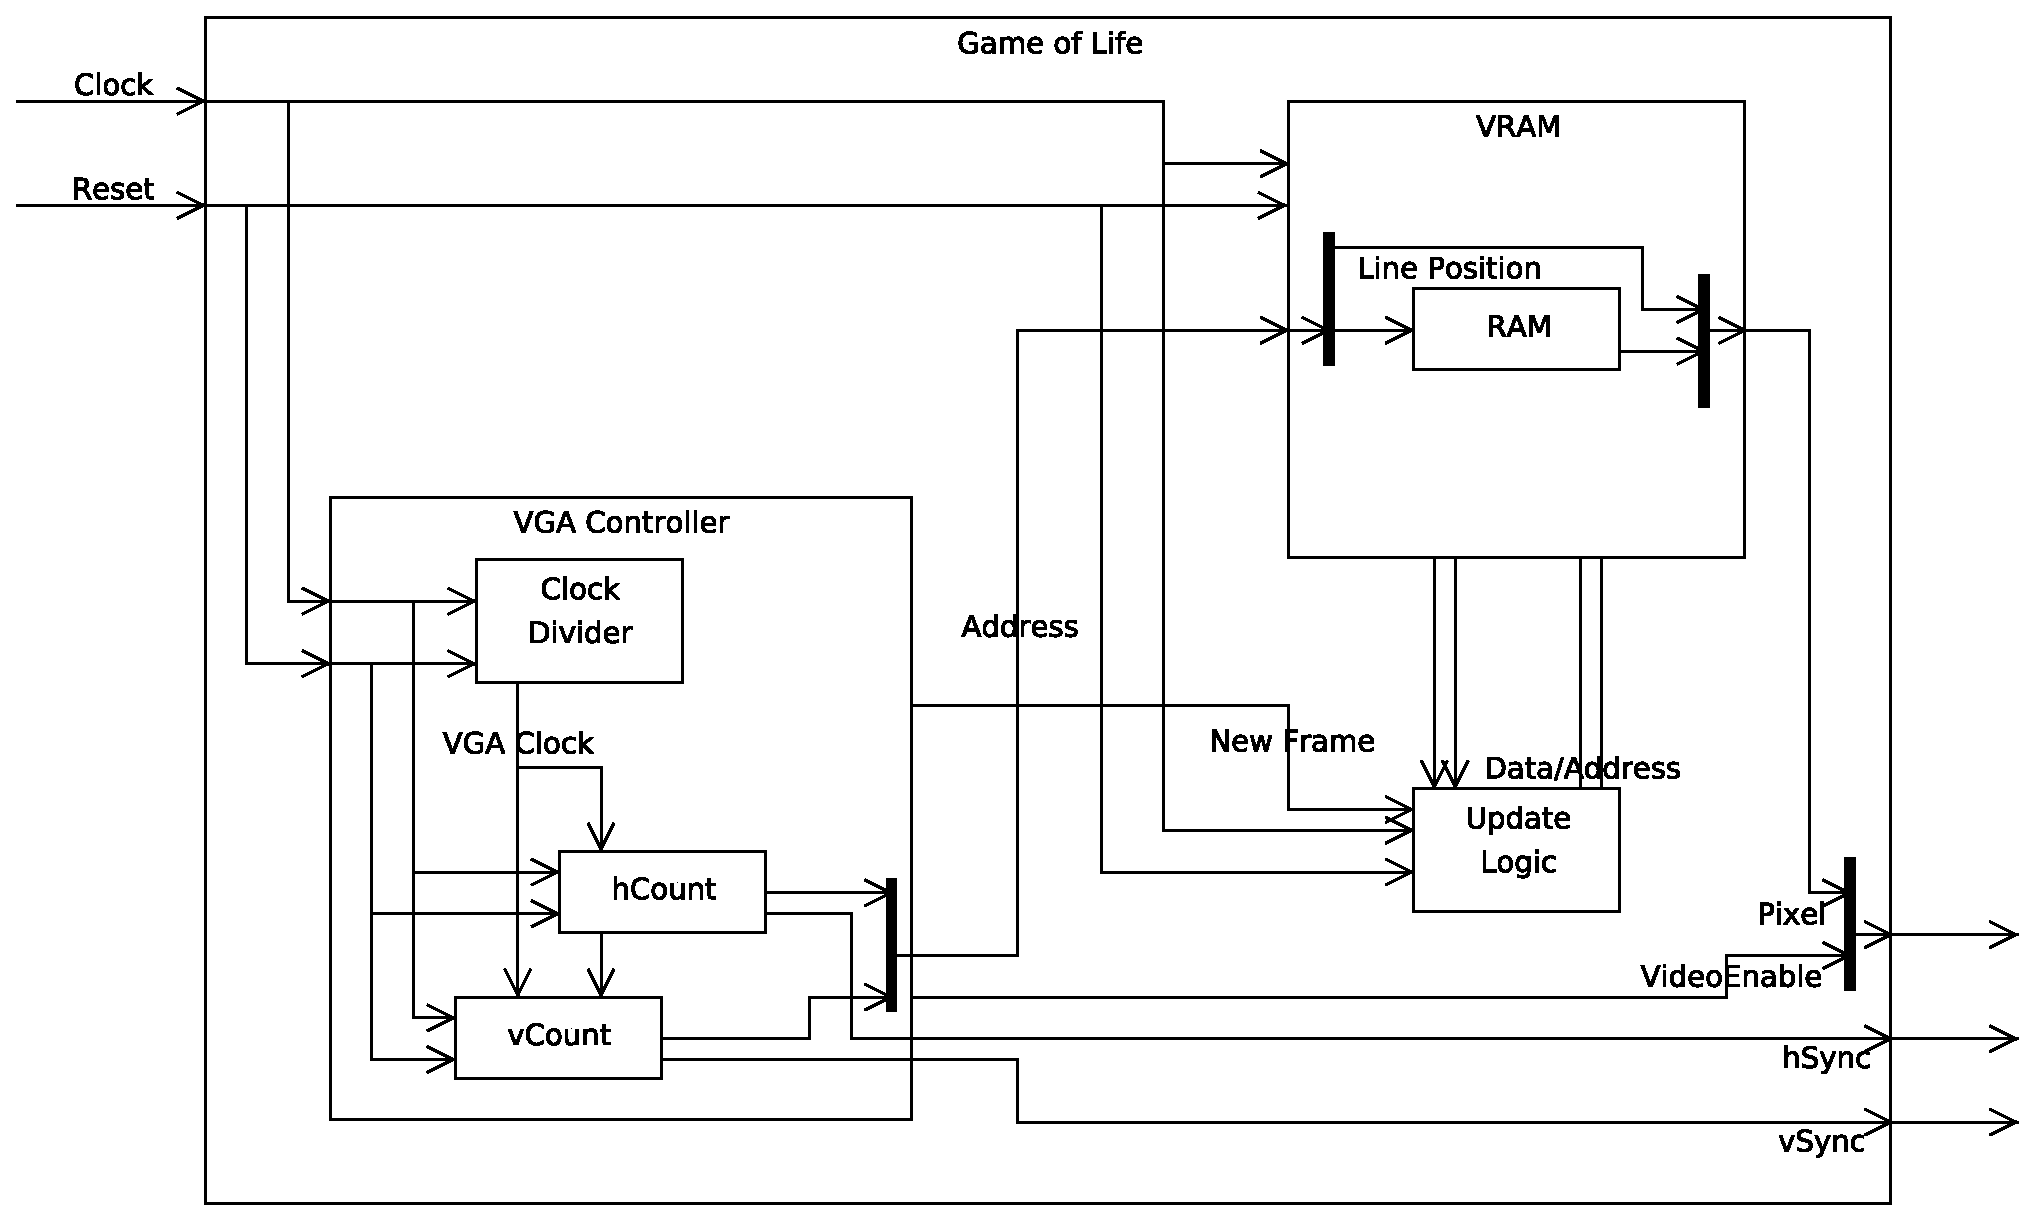
\includegraphics[width=7in]{./media/golBlockDiagram.eps}
\caption{\label{fig:block}Block diagram of Game of Life project.}
\end{figure}

\begin{figure}
\centering
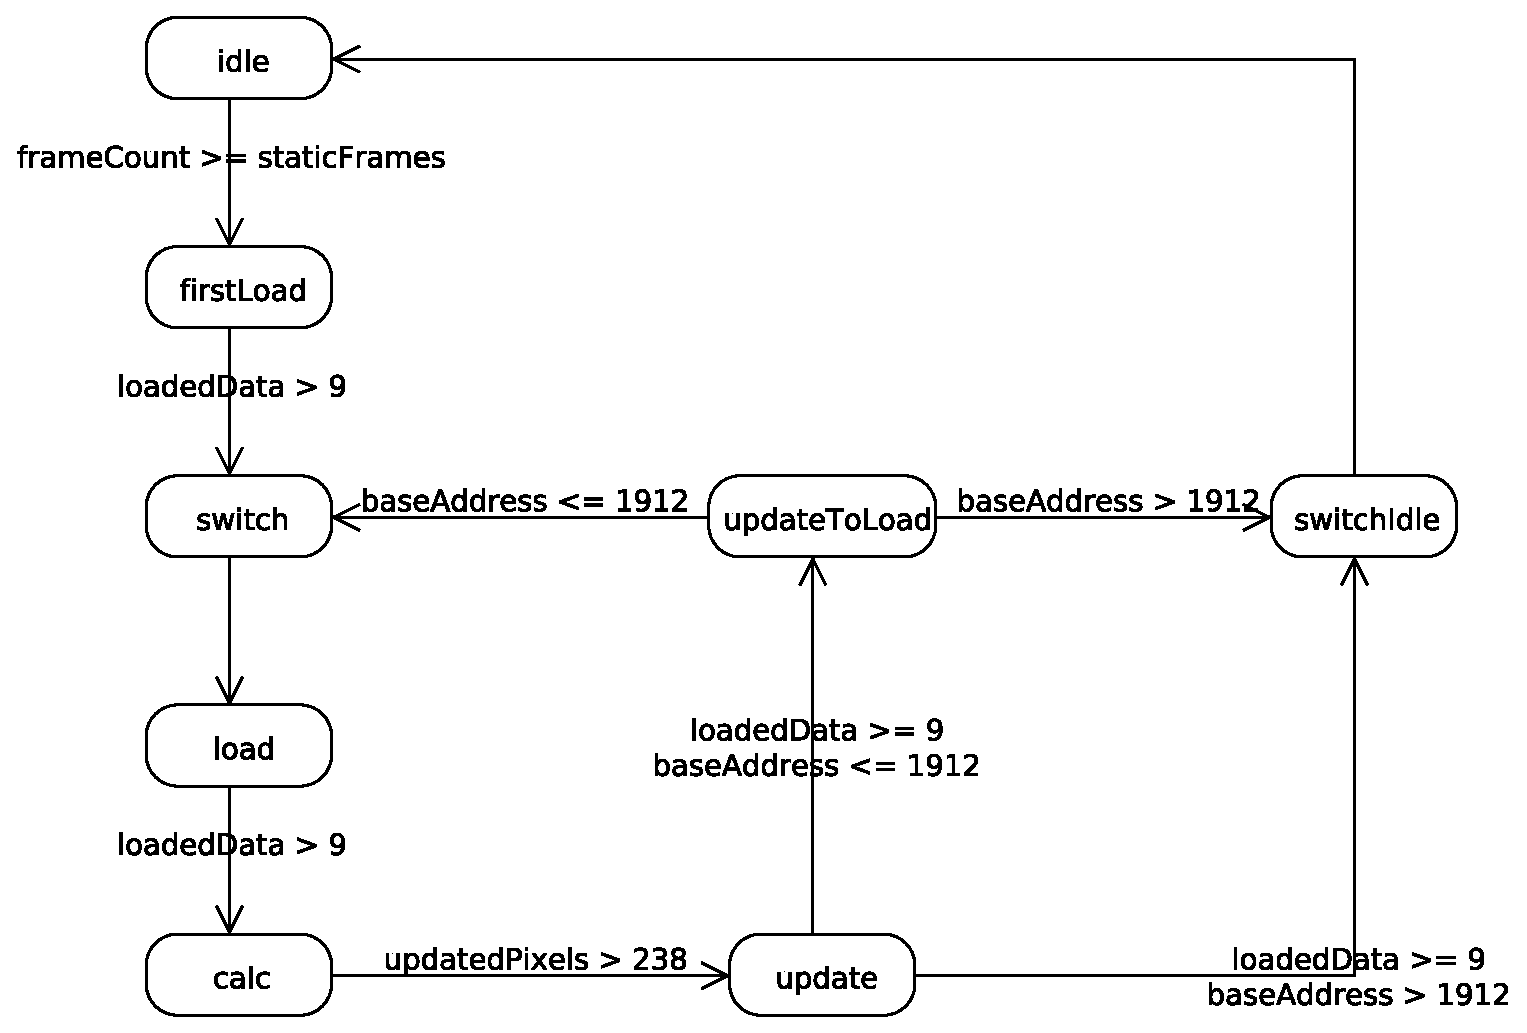
\includegraphics[width=7in]{./media/stateDiagram.eps}
\caption{\label{fig:state}State machine used to update the play field.}
\end{figure}

\begin{figure}
\centering
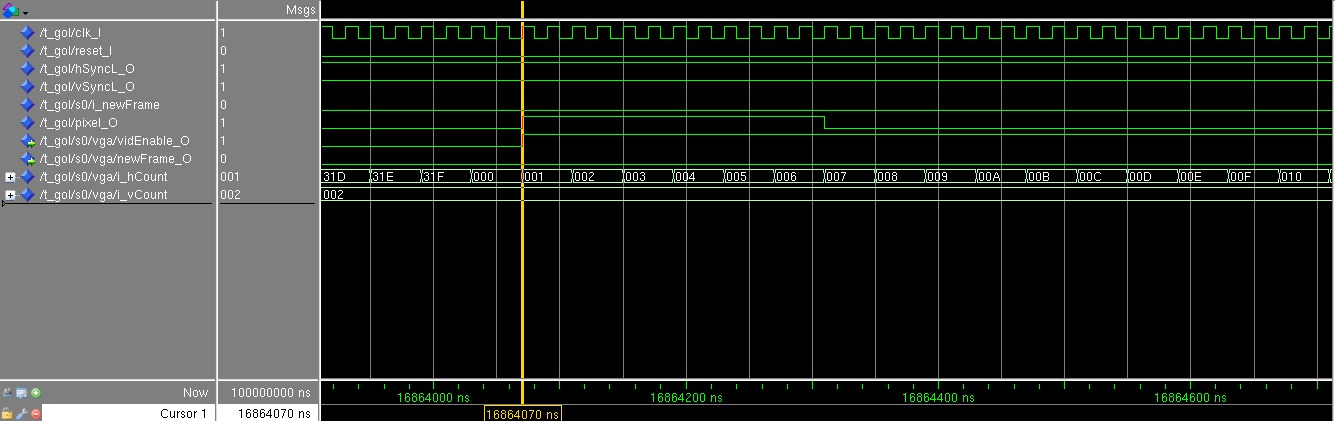
\includegraphics[angle=90, height=9in]{./media/blinker_1.jpg}
\caption{\label{fig:blinker1}Memory is initialized as a 3x1 blinker in row 1, columns 0-2. This figure shows the initial memory block being displayed. HSync is offset by one for RAM access, VSync is at 2 because each pixel is shown twice.}
\end{figure}

\begin{figure}
\centering
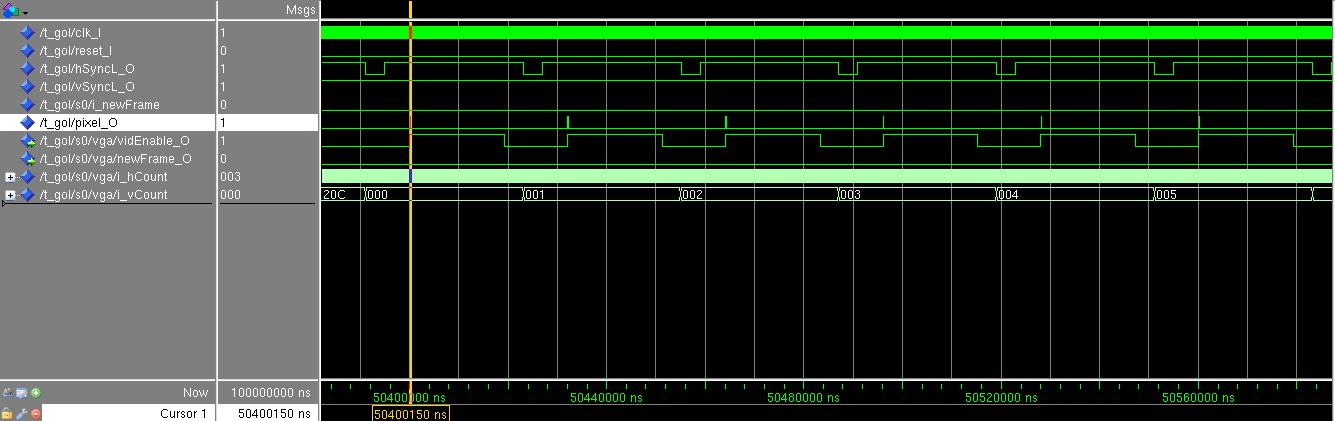
\includegraphics[angle=90, height=9in]{./media/blinker_2.jpg}
\caption{\label{fig:blinker2}This is a zoomed out view of the next figure. It shows the flipped blinker 3 blocks tall (6 pixels) and 1 block wide.}
\end{figure}

\begin{figure}
\centering
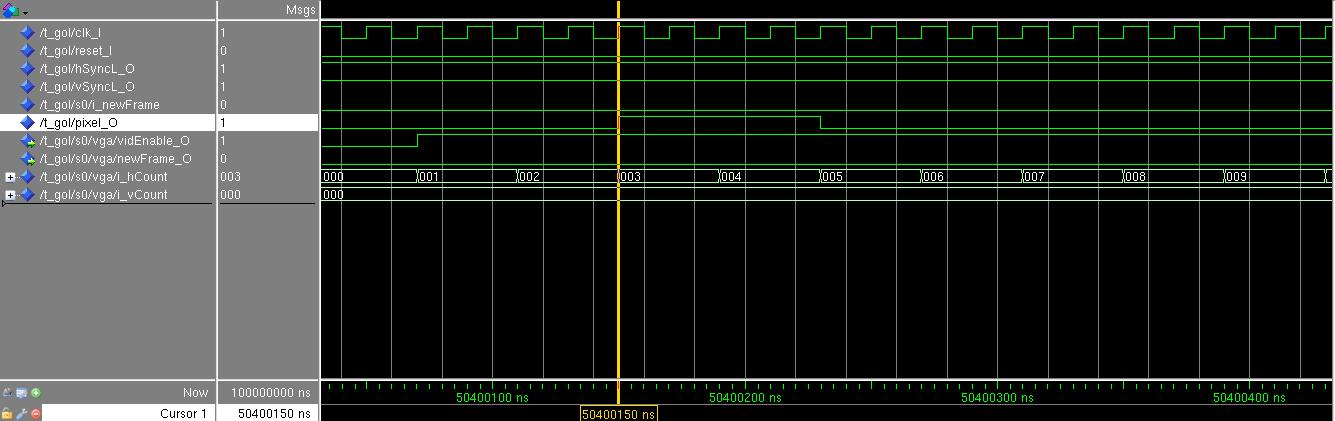
\includegraphics[angle=90, height=9in]{./media/blinker_3.jpg}
\caption{\label{fig:blinker3}Zoomed in view of Figure~\ref{fig:blinker2} showing that the pixel is on for 2 hCounts.}
\end{figure}

\begin{figure}
\label{fig:blinker4}
\centering
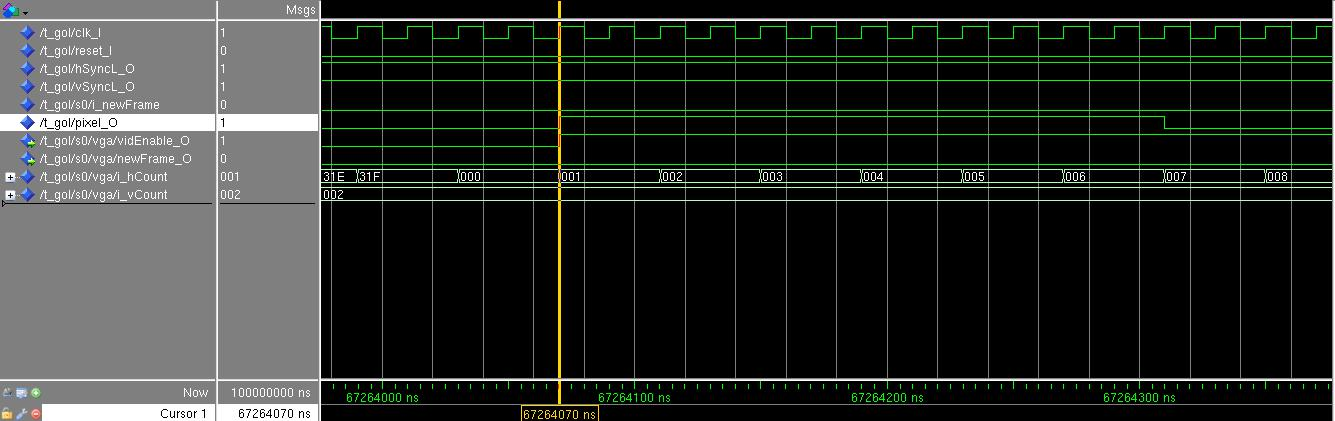
\includegraphics[angle=90, height=9in]{./media/blinker_4.jpg}
\caption{\label{fig:blinker4}The blinker has completed its cycle and displays the same configuration as Figure~\ref{fig:blinker1}.}
\end{figure}

\end{document}
